\documentclass[12pt]{article}

\usepackage[dvips,letterpaper,margin=0.75in,bottom=0.75in]{geometry}
\usepackage{cite}
\usepackage{slashed}
\usepackage{graphicx}
\usepackage{mathtools}
\usepackage{amsmath}
\usepackage{amssymb}
\usepackage{braket}
%\usepackage[american,fulldiode]{circuitikz}
\usepackage{tikz}
\usepackage{arydshln}

\begin{document}

\title{PHY 130B \\ Lecture Notes F: \\
Flavor Symmetry\\}
\author{Michael Mulhearn}

\maketitle

\newcounter{exercise}
\setcounter{exercise}{0}

\newcommand{\exercise}{
\stepcounter{exercise}
\noindent
{\bf Exercise F.\theexercise:}
}

\section{Discrete Symmetries}

\subsection*{Parity}

Parity transforms a three-vector $\mathbf{x} \to -\mathbf{x}$ (by definition).\\[6pt]
In $O(3)$:
\begin{equation*}
  P = \begin{pmatrix} -1 & 0 & 0 \\ 0 & -1 & 0 \\ 0 & 0 & -1 \end{pmatrix}
  = -(I)
\end{equation*}
Notice that $P^2=I$ and so $\{I, P\}$ is a two element group, isomorphic to $\{+1, -1\}$.

The group $O(3)$ is composed entirely of proper rotations with
determinant 1 and improper rotations with determinant -1.
\begin{center}
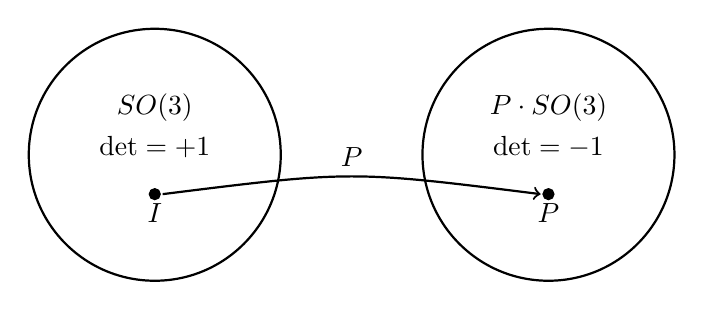
\begin{tikzpicture}
  % SO(3) circle
  \draw[thick] (0,0) circle (1.6cm);
  \node at (0,0.6) {$SO(3)$};
  \node at (0,0.1) {$\det = +1$};
  \filldraw (0,-0.5) circle (2pt) node[below] {$I$};

  % improper rotations circle
  \draw[thick] (5,0) circle (1.6cm);
  \node at (5,0.6) {$P\cdot SO(3)$};
  \node at (5,0.1) {$\det = -1$};
  \filldraw (5,-0.5) circle (2pt) node[below] {$P$};

  % curved arrow over the top
  \draw[->, thick] (0.1,-0.5) .. controls (2.5,-0.2) .. (4.9,-0.5)
    node[midway, above] {$P$};
\end{tikzpicture}
\end{center}
so
\begin{equation*}
  O(3) = \{R, PR \mid P \cdot SO(3)\}
\end{equation*}

The group $SO(3)$ is the representation for angular momentum $l=1$.
While $SO(3)$ does not contain parity $P=-I$, they both act on the same
vector space $R^3$, and for $\vec{x} \in R^3$ we have:
$$P\vec{x} = -I \vec{x} = -\vec{x}$$
and so we say that $l=1$ has negative parity
$$P = -1 \quad \quad (l=1)$$
or we can write:
$$L^P=1^-$$

Suppose $x \in V$ and $y \in W$ have negative parity so:
$$Px = -x, \quad Py = -y$$
then:
\begin{align}
(P \otimes P)(x \otimes y) &= (Px) \otimes (Py) \\
  &= (-x) \otimes (-y) \\
  &= x \otimes y \\
\end{align}
So $x \otimes y$ has postive parity.  We build the $l=2$
representation from $l=1$ via:
$$1^- \otimes 1^- = 2^+ \oplus 1^+ \oplus 0^+ $$
from which we see that $l=2$ has positive parity.  Using induction we conclude:
$$P=(-1)^l$$
You might notice there are $1^+$ representations as well, and this is
a psuedovector (such as $\vec{r} \times {p}$) Does its existence make
this entire argument moot?  No, because we don't build the $l=1$ representation from
$1\otimes1$!
If you don't like this argument, you can also check the spherical harmonics, and indeed, they have:
$$P=(-1)^l$$
exactly as we have argued here.

%%=============================================================
%\pagelabel{12}
%%=============================================================
\section*{Parity Operator for Spinors}

Next we will determine the parity operator for spin one-half
particles, which are represented by $SU(2)$.  We know that $l=1$ is
represented by $SO(3)$ and that there is a Lie algebra
isomorphism $$\mathfrak{su}(2) \cong \mathfrak{so}(3)$$.  But this
helps us not all, because $P$ is not contained in $SO(3)$.  We are not
going to determine parity that way.  Just as for $l=1$, we need
geometric input $\vec{x}=-\vec{x}$ to determine $P$.

What we do have is the Dirac equation.  Parity, you may recall, is a
member of the Lorentz Group, and the Dirac equation is invariant under
Lorentz transformations, so it must be invariant under parity.
Therefore, we can constraint the parity operator for spin one half
particles:
$$P \psi = \psi', \quad \quad P \psi' = \psi$$
by requiring:
$$i (\gamma^\mu \partial_{\mu'}-m) \psi' \iff i (\gamma^\mu \partial_\mu-m) \psi$$
The necessary geometric intput comes as:
$$\frac{\partial}{\partial x'}= -\frac{\partial}{\partial x} \quad
\frac{\partial}{\partial y'}= -\frac{\partial}{\partial y} \quad
\frac{\partial}{\partial z'}= -\frac{\partial}{\partial z} \quad
\frac{\partial}{\partial t'}= \frac{\partial}{\partial t}
$$
or equivalently
$$\partial_i' = - \partial_i, \quad \partial_0' = \partial_0$$
In the exercises, you will show that:
\begin{equation}
\label{eqn:parity-trick}
\gamma^0 \gamma^\mu \partial_\mu' = \gamma^\mu \gamma^0 \partial_\mu
\end{equation}
Returning to the Dirac equation, we now have:
\begin{align*}
   (i\gamma^\mu \partial_{\mu'}-m) \psi' &= 0 \\
  \gamma^0 i (\gamma^\mu \partial_{\mu'}-m) P \psi &= 0 \\
   (i\gamma^\mu \partial_{\mu}-m) \gamma^0 P \psi &= 0 \\
\end{align*}
which recovers the unprimed Dirac equation provided:
\begin{align}
  \gamma^0 P &= \alpha I \\
  (\gamma^0)^2 P &= \alpha \gamma^0 \\
  P &= \alpha \gamma^0 \\
\end{align}
But then
$$P^2 = 1 \implies \alpha^2 = 1$$
so
$$P = \pm \gamma^0$$
and that is as far as the Dirac Equation goes.  We simply have to
choose a convention for this sign, and we take:
\begin{equation}
P = \gamma^0
\end{equation}
You'll show in the exercises that this amounts to setting parity of
spin one-half fermions to +1, and antifermions to -1. Since fermions
and anti-fermions are always produced in pairs, our sign convention
has no physical consquence.\\

\exercise (*) Verify the identity in Equation~\ref{eqn:parity-trick} \\

\exercise (*) Recall that a particle at rest has a bispinor of form:
$$\psi_P = \begin{pmatrix} \phi \\ 0 \end{pmatrix}$$
and an anti-particle at rest:
$$\psi_A = \begin{pmatrix} 0 \\ \phi \end{pmatrix}$$
where $\phi$ is a spinor.  Show that by our convention:
$$P \psi_P = \psi_P$$
and 
$$P \psi_A = -\psi_A$$

\section*{Charge Conjugation}

The Dirac equation predicts the existence of anti-particles with the
same mass and opposite charge of a particle.  To determine the charge
conjugation operator, which turns a particle into its antiparticle, we
need the Dirac equation to include the electric charge, though an
$E\&M$ interaction.  We'll use the minimal substitution from E\&M:
$$p_\mu \to p_\mu - q A_\mu \implies i \partial_\mu \to i \partial_\mu - qA_\mu$$
where
$$A_\mu = (\phi, \mathbf{A})$$
is the four potential.  The Dirac equation becomes:
\begin{equation}
\label{eqn:dirac-minsub}
\gamma^\mu (i \partial_{\mu} - q A_\mu) \psi = m \psi
\end{equation}
In the exercises, you will show that the charge conjugation operator is:
\begin{equation}
\label{eqn:charge-conjugation}
C(\psi) = i \gamma^2 \psi^*
\end{equation}
Note that
$$C(\alpha \psi) = \bar{\alpha} C(\psi)$$
which says that $C$ is anti-linear.\\

\exercise (*) Show that:
$$\gamma^2 (\gamma^u)^* = -\gamma^u \gamma^2\\[5pt]$$

\exercise (*) Derive Equation~\ref{eqn:charge-conjugation} as follows.
Take the complex conjugate of the Dirac equation with minimal
substituion from Equation~\ref{eqn:dirac-minsub}, and multiply both
sides by $\gamma^2$.  Using the identity from the previous exercise, you should be able to show that:
$$\gamma^\mu (i \partial_{\mu} + q A_\mu) (\gamma^2 \psi^*) = m (\gamma^2 \psi^*)$$
This shows (note the change of sign before $q$) that:
$$C(\psi) = \alpha \gamma^2 \psi^*$$
where $\alpha$ is a complex number.  We put $\alpha=i$ by convention.

\exercise For $C(\psi) = \alpha \gamma^2 \psi^*$ show that:
$$C^2 = -|\alpha|^2$$

\subsection*{Charge Conjugation for Spinors}
The charge conjugation operator
\begin{equation*}
  C(\psi) = i\gamma^2\psi^*
\end{equation*}
acts on a bispinor which describes either a particle or an
antiparticle.  A particle at rest has the form:
$$\psi_p = \begin{pmatrix} \chi \\ 0 \end{pmatrix}$$
and an anti-particle at rest has the form:
$$\psi_a = \begin{pmatrix} 0 \\ \chi \end{pmatrix}$$
Calculating:
\begin{equation*}
  C(\psi_p) = i\gamma^2 \, \psi_p^* =
  \begin{pmatrix} 0 & -i\sigma_2 \\ i\sigma_2 & 0 \end{pmatrix}
  \begin{pmatrix} \chi^* \\ 0 \end{pmatrix}
  \quad\Rightarrow\quad
  = 
  \begin{pmatrix} 0 \\ i \sigma_2 \chi^* \end{pmatrix}
\end{equation*}
We see that the charge conjugation operator for a spinor is:
\begin{equation}
\label{eqn:c_spinor}
  C(\chi) = i\sigma_2 \chi^*
\end{equation}
or writing it out explicitly:
\begin{align*}
  C(\chi) &= i\begin{pmatrix} 0 & -i \\ i & 0 \end{pmatrix}\chi^* \\[7pt]
  &= \phantom{i}\begin{pmatrix} 0 & 1 \\ -1 & 0 \end{pmatrix}\chi^* 
\end{align*}

\exercise Show that
$$C^2(\chi) = -\chi$$

\exercise Show that
$$C^-1(\chi) = -i\sigma_2 \chi^*$$


\section{Isospin Symmetry}

One of the most striking features of the nuclear strong force is that
it evidently does not distinguish between neutrons and protons,
drawing both of them together tightly into a dense atomic nucleus.
Protons have quark content $uud$ and neutrons $udd$ so our modern
understanding of this symmetry is best understood as a symmetry
between up quarks and down quarks.  Evidently, the nuclear strong
force is unchanged by rotations that mix up quarks and down quarks:
\begin{equation*}
  \begin{pmatrix} u' \\ d' \end{pmatrix}
  = U
  \begin{pmatrix} u \\ d \end{pmatrix},
  \qquad U \in SU(2)
\end{equation*}
You might wonder why we consider $SU(2)$ and not $U(2)$ but the latter
differs from the former by only an overall phase, and doesn't mix $u$
and $d$, and is therefore not considered part of this symmetry.

Because $SU(2)$ is also the fundamental symmetry of spin one-half, we
refer to this new symmetry as isospin.  Except for being an $SU(2)$
symmetry, it has nothing to do with spin!

\subsection*{SU(2) and the generators of Isospin}

An element $U$ of $SU(2)$ can be written as
\begin{equation*}
  U =
  \begin{pmatrix} \alpha & \beta \\ -\beta^* & \alpha^* \end{pmatrix}
\end{equation*}
with $\alpha,\beta \in \mathcal{C}$ and the constraint that:
$$\det(U) = |\alpha|^2 + |\beta|^2 = 1.$$
We already calculated the three generators associated with $SU(2)$ in
the context of spin, and labeled them $S_x$, $S_y$, and $S_z$.
Isospin rotations are in an abstract $u$ and $d$ space, which has
nothing to do with $x$,$y$, and $z$.  Therefore, we label the Isopsin
generators more abstractly:
\begin{equation}
  I_1 = \frac{1}{2}\sigma_1 = \frac{1}{2}\begin{pmatrix} 0 &  1 \\ 1 &  0 \end{pmatrix}, \qquad
  I_2 = \frac{1}{2}\sigma_2 = \frac{1}{2}\begin{pmatrix} 0 & -i \\ i &  0 \end{pmatrix}, \qquad
  I_3 = \frac{1}{2}\sigma_3 = \frac{1}{2}\begin{pmatrix} 1 &  0 \\ 0 & -1 \end{pmatrix}
\end{equation}
The $u$ quark and $d$ quark are represented as:
$$ u = \begin{pmatrix} 1 \\  0 \end{pmatrix}, \qquad
d = \begin{pmatrix} 0 \\  1 \end{pmatrix}, \qquad
$$
From which we see:
$$I_3 \, u \quad = \; \frac{1}{2}\begin{pmatrix} 1 &  0 \\ 0 & -1 \end{pmatrix}
\, \begin{pmatrix} 1 \\  0 \end{pmatrix} \; = \;  
\phantom{-}\frac{1}{2} \begin{pmatrix} 1 \\  0 \end{pmatrix} = \phantom{-}\frac{1}{2} u 
$$
and 
$$I_3 \, d \quad = \; \frac{1}{2}\begin{pmatrix} 1 &  0 \\ 0 & -1 \end{pmatrix}
\, \begin{pmatrix} 0 \\  1 \end{pmatrix} \; = \; 
-\frac{1}{2} \begin{pmatrix} 0 \\  1 \end{pmatrix} = -\frac{1}{2} d 
$$
from which we see that $u$ and $d$ have third-component of Isospin:\\
\begin{center}
\begin{tabular}{ll}
\hline
  & $I_3$ \\
\hline
$u$ & $+\frac{1}{2}$ \\
$d$ & $-\frac{1}{2}$ \\
\hline
\end{tabular}
\end{center}
We also have Isospin raising and lowering operators defined as:
\begin{equation*}
  I_+ = I_1 + i I_2 = \begin{pmatrix} 0 & 1 \\ 0 & 0 \end{pmatrix}, \qquad
  I_- = I_1 - i I_2 = \begin{pmatrix} 0 & 0 \\ 1 & 0 \end{pmatrix}, \qquad
\end{equation*}
From which we see that:
$$I_+ \, u \, = \, 0, \quad I_+ \, d \, = \, u, \quad 
I_- \, u \, = \, d, \quad I_- \, d \, = \, 0, \quad$$

\exercise Suppose that a matrix $X$ is diagonalizable, which means
that there is a matrix $A$ such that:
$$A^{-1} X A = \begin{pmatrix} \lambda_1 & & \\ & \lambda_2 & \\ & & \ddots \end{pmatrix}$$
show that:
$$ \det(e^X) = e^{{\rm Tr}(X)}$$
Hint: first show that:
$$\det(e^X) = \det(A^{-1} e^X A) = \det(e^{A^{-1} X A})$$
and then you are well on your way.  This result is quite general, but
the condition that $X$ is diagonalizable makes it easier to show.\\[5pt]

\exercise Use the results of the previous exercise to show that
the generators of $SU(n)$ are traceless.

\subsection{Isospin and anti-particles}

With respect to the Dirac equation, the Isospin of a particle is
irrelevant, and we can simply consider two differents bispinors:
$\psi_u$ for the up quark, and $ \psi_d$ for down quark.  Under charge
conjugation we have:
$$C(\psi_u) = i \gamma^2 \psi_u^*, \quad C(\psi_d) = i \gamma^2
\psi_d^*$$
so in Isospin space we need only take the complex conjugate
to change a particle to an antiparticle:
$$\begin{pmatrix} \bar{u} \\ \bar{d}\end{pmatrix}
= \begin{pmatrix} u \\ d\end{pmatrix}^*
$$
and so for a unitary transformation for quarks:
$$\begin{pmatrix} u' \\ d' \end{pmatrix} =     
   \begin{pmatrix}\alpha & \beta \\ -\beta^* & \alpha^* \end{pmatrix}
\begin{pmatrix} u \\ d \end{pmatrix}$$
we take the complex conjugage:
$$\begin{pmatrix} u' \\ d' \end{pmatrix}^* =     
   \begin{pmatrix}\alpha & \beta \\ -\beta^* & \alpha^* \end{pmatrix}^*
\begin{pmatrix} u \\ d \end{pmatrix}^*$$
to obtain the corresponding unitary operation for antiquarks:
$$\begin{pmatrix} \bar{u}' \\ \bar{d}' \end{pmatrix} =     
   \begin{pmatrix}\alpha^* & \beta^* \\ -\beta & \alpha \end{pmatrix}
\begin{pmatrix} \bar{u} \\ \bar{d} \end{pmatrix}$$
Thus, the antiquarks transform differently under the same symmetry
operation, and so the generators will be different, which promises to
be quite a hassle.  Fortunately, in the exercises, you will show that
if, inspired by charge conjugation operator for spinors, we redefine
the anti-quark doublet as:
$$
-i \sigma(2) \begin{pmatrix} u \\ d \end{pmatrix}^*
=
\begin{pmatrix} 0 & -1 \\ 1 & 0 \end{pmatrix} \,
\begin{pmatrix} \bar{u} \\ \bar{d} \end{pmatrix}^*
=
\begin{pmatrix} -\bar{d} \\ \bar{u} \end{pmatrix}
$$
Thus we have:
$$ \bar{u} = \begin{pmatrix} 0 \\  1 \end{pmatrix}, \qquad
\bar{d} = \begin{pmatrix} -1 \\  0 \end{pmatrix}, \qquad
$$
Also in the exercises, you will show that $\bar{u}$ and $\bar{d}$ have third-component of Isospin:\\
\begin{center}
\begin{tabular}{ll}
\hline
  & $I_3$ \\
\hline
$\bar{u}$ & $-\frac{1}{2}$ \\
$\bar{d}$ & $+\frac{1}{2}$ \\
\hline
\end{tabular}
\end{center}
and
\begin{equation}
  \label{eqn:isospin-antiparticles}
  I_+ \, \bar{u} \, = \, -\bar{d}, \quad I_+ \, \bar{d} \, = \, 0, \quad
  I_- \, \bar{u} \, = \, 0, \quad I_- \, \bar{d} \, = \, -\bar{u} 
\end{equation}
Notice that the Isospin quantum numbers change sign for antiparticles.\\[5pt]

\exercise (*) For an element of $SU(2)$ written as:
$$U = \begin{pmatrix} \alpha & \beta \\ -\beta^* & \alpha^* \end{pmatrix}$$
and the transformation
$$S = i \sigma_2$$
show that
$$S^{-1} = -i \sigma_2$$
and
$$S^{-1} U S = U^*$$


\exercise Use the results of the previous exercise to show that if
$$\psi' = U^* \psi$$
then
$$S \psi' = U S \psi$$
which shows that
$$S \begin{pmatrix} \bar{u} \\ \bar{d} \end{pmatrix}
= \begin{pmatrix} -\bar{d} \\ \bar{u} \end{pmatrix}
$$
transforms the same way as:
$$\begin{pmatrix} u \\ d \end{pmatrix}$$

\exercise  Show that $I_3 \bar{u}$ and $I_3 \bar{d}$ are consistent with the results in the table above Equation~\ref{eqn:isospin-antiparticles}.\\[5pt]

\exercise Verify Equation~\ref{eqn:isospin-antiparticles}.\\[5pt]

\section*{The Pions and Eta}

Using Isopsin, we can start to make sense of the mesons, composed
of a quark and an antiquark.  We'll consider the lightest quarks $u$
and $d$.  The lighest mesons will have $l=0$ and $s=0$, and so $j=0$.
In the exercises you will show that they have parity $P=-1$, so we
write:
$$j^P = 0^-$$
and call these the light pseudoscalar mesons.

Just as with angular momentum, we start from an extreme state, the positive pion:
$$\pi^+ = u \bar{d}$$
which ha $I_3 = +1$.  Applying $I_-$ we calculate:
$$I_- \pi^+ = I_- u \bar{d} = d \bar{d} - u \bar{u}$$
to normalize the resulting state we must divide by $\sqrt{2}$ and we obtain the neutral pion:
$$\pi^0 = \frac{1}{\sqrt{2}} (d \bar{d} - u \bar{u})$$
Applying $I_-$ again calculate:
$$I_- \pi^0 = I_- \frac{1}{\sqrt{2}} (d \bar{d} - u \bar{u}) = -\sqrt{2} \, d \bar{u}$$
and again we have to divide by $\sqrt{2}$ to obtain the normalized negative pion:
$$\pi^- = - d \bar{u} $$
Hitting the $pi^-$ with $I_-$ yields 0, as we have walked through the $I=1$ triplet:
$$I_- \ket{I=1, I_3=+1} = \sqrt{2} \ket{I=1, I_3=0} $$
and 
$$I_- \ket{I=1, I_3=0} = \sqrt{2} \ket{I=1, I_3=-1} $$
with the factors of $\sqrt{2}$ exactly as we found (we needed to divide
by the same factor to get a normalized state.

The remaining state is the Eta:
$$\eta = \frac{1}{\sqrt{2}} (d \bar{d} + u \bar{u})$$
in the exercises you'll show that it is othogonal to the $\pi^0$ and a singlet.\\[5pt]


\exercise (*) Show that mesons with $l=0$ and $s=0$ have parity $P=-1$.
There are three contributions to the parity, make sure you account
for all three.\\[5pt]

\exercise  (*) Write the $\pi^0$ and $\eta$ as vectors in the 2-D subspace
with bases $\{u \bar{u}, d \bar{d}\}$.  Show that they are orthogonal.\\[5pt]

\exercise  Apply $I_-$ and $I_+$ to the $\eta$ and show that the result is zero.  This shows that $\eta$ is the singlet.\\[5pt]

\section{Flavor Symmetry}

The flavor symmetry between the $u$ and $d$ quarks can be expanded to include
the $s$ quark:
\begin{equation*}
  \begin{pmatrix} u' \\ d' \\ s' \end{pmatrix}
  = U
  \begin{pmatrix} u \\ d \\ s \end{pmatrix},
  \qquad U \in SU(3)
\end{equation*}

\section*{The Lie Algebra of $SU(3)$}

We wish to find the generators of $SU(3)$, i.e.\ to find the Lie
algebra $\mathfrak{su}(3)$. We could work out an explicit
parameterization of $SU(3)$ and differentiate, but that is painful.
Instead, we will use what we already know.\\[6pt]


Elements of $SU(3)$ are $(3\times 3)$
complex unitary matrices with $\det(U)=1$.  Unitarity provides $3\times 3$ constraints, and the determinant 1.  Thus the total number of free parameters is:
$$N = 3\times 3\times 2 - 3\times 3 - 1 = 8$$
Thus we know that $su{3}$ has {\bf eight generators.}
Just as for $\mathfrak{su}(2)$, the generators are
\textbf{traceless Hermitian} matrices.  Thus, if we find 8 linearly
independent traceless Hermitian $3 \times 3$ matrices, we have found
our generators, and a basis for $su{3}$.

\section*{A Basis for $\mathfrak{su}(3)$: The Gell-Mann Matrices}

We split the 8 generators into three groups according to the $SU(2)$
subgroup they generate.\\[6pt]

\noindent\textbf{Isospin} ($u\leftrightarrow d$):
\begin{equation*}
  \lambda_1 =
  \begin{pmatrix} 0 & 1 & 0 \\ 1 & 0 & 0 \\ 0 & 0 & 0 \end{pmatrix},\quad
  \lambda_2 =
  \begin{pmatrix} 0 & -i & 0 \\ i & 0 & 0 \\ 0 & 0 & 0 \end{pmatrix},\quad
  \lambda_3 =
  \begin{pmatrix} 1 & 0 & 0 \\ 0 & -1 & 0 \\ 0 & 0 & 0 \end{pmatrix}
\end{equation*}

\noindent\textbf{V-spin} ($u\leftrightarrow s$):
\begin{equation*}
  \lambda_4 =
  \begin{pmatrix} 0 & 0 & 1 \\ 0 & 0 & 0 \\ 1 & 0 & 0 \end{pmatrix},\quad
  \lambda_5 =
  \begin{pmatrix} 0 & 0 & -i \\ 0 & 0 & 0 \\ i & 0 & 0 \end{pmatrix},\quad
  A =
  \begin{pmatrix} 1 & 0 & 0 \\ 0 & 0 & 0 \\ 0 & 0 & -1 \end{pmatrix}
\end{equation*}

\noindent\textbf{U-spin} ($d\leftrightarrow s$):
\begin{equation*}
  \lambda_6 =
  \begin{pmatrix} 0 & 0 & 0 \\ 0 & 0 & 1 \\ 0 & 1 & 0 \end{pmatrix},\quad
  \lambda_7 =
  \begin{pmatrix} 0 & 0 & 0 \\ 0 & 0 & -i \\ 0 & i & 0 \end{pmatrix},\quad
  B =
  \begin{pmatrix} 0 & 0 & 0 \\ 0 & 1 & 0 \\ 0 & 0 & -1 \end{pmatrix}
\end{equation*}
This is 9 matrices, one more than we need, and the reason is that $\lambda_3$, $A$, and $B$ are not independent, in fact:
$$\lambda_3 = A - B$$
We want to keep $\lambda_3$, as this is the third component of Isospin, a familiar observable.  We want to find a commuting observable, which should be of form:
$$\begin{pmatrix} 1 & 0 & 0 \\ 0 & 1 & 0 \\ 0 & 0 & x \end{pmatrix}$$
and a linear combination of $A$ and $B$.  We find that $A+B$ does the trick and define:
\begin{equation*}
\lambda_8 =
  \frac{1}{\sqrt{3}} 
  \begin{pmatrix} 1 & 0 & 0 \\ 0 & 1 & 0 \\ 0 & 0 & -2 \end{pmatrix}
\end{equation*}
These 8 matrices are traceless and Hermitian, and are linearly
independent. They form a basis for $\mathfrak{su}(3)$.  
For two $n\times n$ matrices $A$ and $B$, we can define their inner product by:
$$\braket{A \mid B} = {\rm Tr}(A^\dagger\,B)$$
The Gell-Mann matrices are orthogonal wrt this inner product:
\begin{equation}
\label{eqn:lambda-traces}
  \mathrm{Tr}(\lambda_a \lambda_b) = 2 \delta_{ab}
\end{equation}


\exercise (*) Show that the generators $\{\lambda_i\}$ of $SU(3)$
satisfy Equation~\ref{eqn:lambda-traces}. In principle this is 64
calculations, but we can reduce this by being clever. In fact, we need
only calculate directly:
\begin{equation*}
  \mathrm{Tr}(\lambda_1^2),\quad
  \mathrm{Tr}(\lambda_1\lambda_2),\quad
  \mathrm{Tr}(\lambda_1\lambda_4),\quad
  \mathrm{Tr}(\lambda_1\lambda_8),\quad
  \mathrm{Tr}(\lambda_8^2)
\end{equation*}
then argue the rest follow from the cyclic property of the trace,
cyclic rotations of $(u,d,s)$, cyclic rotations of $(\sigma_1,
\sigma_2, \sigma_3)$ (which follows from cyclic rotations of $x$,$y$
and $z$), and $\lambda_8 \propto \lambda_A + \lambda_B$.\\[5pt]

\exercise Let's formalize one of the cyclic arguments from the
previous exercise. Find the matrix $S$ that implements the cyclic
permutation $u\to d\to s\to u$, and show it is unitary. Then show
that for a unitary $S$ and $\lambda' \equiv S^\dagger \lambda S$:
\begin{equation*}
  \mathrm{Tr}(\lambda_a'\,\lambda_b') = \mathrm{Tr}(\lambda_a\,\lambda_b)
\end{equation*}
from which the flavor part of the cyclic argument follows directly.\\[5pt]

\exercise To complete the cyclic argument from the previous problems,
we need to find $S$ such that:
$$S^\dagger \sigma_1 S = \sigma_2$$
and so on.  The solution is:
$$S \; = \; R_x(\pi/2) \, R_z(\pi/2) =
\exp(i\sigma_1 \pi/4) \, \exp(i\sigma_3 \pi/4)
=
\frac{1}{2}\begin{pmatrix} 1+1 & 1+i \\ -1+i & 1+i \end{pmatrix}$$
Show that indeed:
$$S^{-1} \sigma_1 S = \sigma_2$$
  

\section*{Hypercharge}

We have two diagonal generators, $\lambda_3$ and $\lambda_8$, which we use to define observables.
We first define
\begin{equation*}
  T_3 = \tfrac{1}{2}\lambda_3 = \frac{1}{2}\begin{pmatrix} 1 & 0 & 0 \\ 0 & -1 & 0 \\ 0 & 0 & 0 \end{pmatrix}
\end{equation*}
which is the third component of isospin in our higher dimensional space.  Next we define:
\begin{equation*}
  Y = \tfrac{1}{\sqrt{3}}\lambda_8 = \frac{1}{3}\begin{pmatrix} 1 & 0 & 0 \\ 0 & 1 & 0 \\ 0 & 0 & -2 \end{pmatrix}
\end{equation*}
which is called hypercharge.  By construction, hypercharge ($Y$) and
the third-component of isospin ($I_3$) commute, so they are compatible
observables.  They are also othogonal, in the sense that:
$$Tr(T_3 Y) = 0$$
so the quantum numbers for isospin and hypercharge are independent.

The quantum numbers for the $u$,$d$, and $s$ quarks are along the diagonals, e.g.
$$Y d = \frac{1}{3}\begin{pmatrix} 1 & 0 & 0 \\ 0 & 1 & 0 \\ 0 & 0 & -2 \end{pmatrix}
\begin{pmatrix} 0 \\ 1 \\ 0  \end{pmatrix} = \frac{1}{3} d
$$
so we can tabulate $Y$ and $T_3$ as:
\begin{center}
  \begin{tabular}{c|ccc}
  & $T_3$ & $Y$ & $Q$ \\
  \hline
  $u$ & $+\tfrac{1}{2}$ & $+\tfrac{1}{3}$ & $+\tfrac{2}{3}$ \\[4pt]
  $d$ & $-\tfrac{1}{2}$ & $+\tfrac{1}{3}$ & $-\tfrac{1}{3}$ \\[4pt]
  $s$ & $0$             & $-\tfrac{2}{3}$ & $-\tfrac{1}{3}$ \\
\end{tabular}
\end{center}
and the quantum numbers change sign for antiparticles so:
\begin{center}
  \begin{tabular}{c|ccc}
  & $T_3$ & $Y$ & $Q$ \\
  \hline
  $\bar{u}$ & $-\tfrac{1}{2}$ & $-\tfrac{1}{3}$ & $-\tfrac{2}{3}$ \\[4pt]
  $\bar{d}$ & $+\tfrac{1}{2}$ & $-\tfrac{1}{3}$ & $+\tfrac{1}{3}$ \\[4pt]
  $\bar{s}$ & $0$             & $+\tfrac{2}{3}$ & $+\tfrac{1}{3}$ \\
\end{tabular}
\end{center}
Notice that $Q$ (which is only reported here, not predicted) is related to $T_3$ and $Y$ as:
\begin{equation*}
  Q = T_3 + \tfrac{1}{2}Y
\end{equation*}


\section*{Raising and Lowering Operators of $SU(3)$}

$SU(3)$ contains three $SU(2)$ subgroups, each with its own raising
and lowering operators:
\begin{center}
\begin{tabular}{ccc}
  Isospin ($u\leftrightarrow d$) & V-spin ($u\leftrightarrow s$) & U-spin ($d\leftrightarrow s$) \\
  \hline \\[-6pt]
  $T_\pm = \tfrac{1}{2}(\lambda_1 \pm i\lambda_2)$ &
  $V_\pm = \tfrac{1}{2}(\lambda_4 \pm i\lambda_5)$ &
  $U_\pm = \tfrac{1}{2}(\lambda_6 \pm i\lambda_7)$ \\[7pt]
  $T^+d = u$ & $V^+s = u$ & $U^+s = d$ \\
  $T^-u = d$ & $V^-u = s$ & $U^-d = s$ \\
  $T^+\bar{u} = -\bar{d}$ & $V^+\bar{s} = -\bar{u}$ & $U^+\bar{d} = -\bar{s}$ \\
  $T^-\bar{d} = -\bar{u}$ & $V^-\bar{u} = -\bar{s}$ & $U^-\bar{s} = -\bar{d}$ \\
\end{tabular}
\end{center}


\section*{The Eightfold Way}

Using the raising and lowering operators, we find an octet of
particles:

\begin{center}
\begin{tikzpicture}[scale=1.0]

  % Coordinate system:
  % T3 axis horizontal, Y axis vertical
  % pi+ at (-4,0), pi0 at (0,0), pi- at (4,0)
  % K+ at (-2, 3), K0 at (2, 3)
  % K- at (4,-3)... wait: K- has T3=-1/2, so at (2,-3)
  % Kbar0 at (-2,-3)

  % --- Upper kaons (Y=+1) ---
  % K+ : quark content ubar{s}, T3=+1/2 -> x=-2
  \filldraw (-2,3) circle (2pt);
  \node[above] at (-2,3.15) {$K^+$};
  \node[below] at (-2,2.85) {$u\bar{s}$};

  % K0 : quark content dbar{s}, T3=-1/2 -> x=+2
  \filldraw (2,3) circle (2pt);
  \node[above] at (2,3.15) {$K^0$};
  \node[below] at (2,2.85) {$d\bar{s}$};

  % --- Central row (Y=0) ---
  % pi+
  \filldraw (-4,0) circle (2pt);
  \node[above] at (-4,0.15) {$\pi^+$};
  \node[below] at (-4,-0.15) {$u\bar{d}$};

  % pi0
  \filldraw (0,0) circle (2pt);
  \node[above] at (0,0.15) {$\pi^0, \eta_8$};
  \node[below] at (0,-0.15) {$d\bar{d} - u\bar{u}$};
  \node[below] at (0,-0.60) {$d\bar{d} + u\bar{u} - 2 s\bar{s}$};
    
  % pi-
  \filldraw (4,0) circle (2pt);
  \node[above] at (4,0.15) {$\pi^-$};
  \node[below] at (4,-0.15) {$d\bar{u}$};

  % --- Lower kaons (Y=-1) ---
  % Kbar0 : quark content sbar{d}, T3=+1/2 -> x=-2
  \filldraw (-2,-3) circle (2pt);
  \node[below] at (-2,-3.15) {$\bar{K}^0$};
  \node[above] at (-2,-2.85) {$\bar{d}s$};

  % K- : quark content sbar{u}, T3=-1/2 -> x=+2
  \filldraw (2,-3) circle (2pt);
  \node[below] at (2,-3.15) {$K^-$};
  \node[above] at (2,-2.85) {$\bar{u}s$};

  % --- Arrows from pi+ upward ---
  \draw[->] (-3.6,0.75) -- (-2.6,2.25) node[midway, left] {$U^+$};
  \draw[->] (-1.2, 3) -- ( 1.2, 3) node[midway, above] {$T_-$};
  \draw[->] (-1.2, -3) -- ( 1.2, -3) node[midway, above] {$T_-$};
  
  % --- Arrows from pi+ downward ---
  \draw[->] (-3.6,-0.75) -- (-2.6,-2.25) node[midway, left] {$V^-$};

  % --- Arrows along central row ---
  \draw[->] (-3.2,0.2) -- (-0.8,0.2) node[midway, above] {$T_-$};
  \draw[->] (0.8,0.2) -- (3.2,0.2) node[midway, above] {$T_-$};

\end{tikzpicture}
\end{center}
At the center ($T_3=0$, $Y=0$), we find the $pi_0$ from $T_ \pi^+$:
$$d\bar{d} - u\bar{u}$$
plus two more states:
\begin{align*}
  x &\equiv U_+ s \bar{d} = d \bar{d} - s \bar{s} \\
  y &\equiv V_- u \bar{s} = s \bar{s} - u \bar{u} \\
\end{align*}
however, these are not orthogonal, because:
$$x + y = d\bar{d} - u\bar{u} = \pi^0$$
so we take the orthogonal part:
$$x-y = d\bar{d} - u\bar{u} - 2 s \bar{s}= \eta_8$$

This leaves a singlet:
$$\eta_1 = d\bar{d} + u\bar{u} + s \bar{s}= \eta_1$$

\exercise (*) Show that the $\eta_1$ is indeed a singlet by hitting it
with all six raising and lowering operators and getting zero.\\[5pt]

\section*{Big Picture: $SU(3)$ Flavor Symmetry}

$SU(3)$ flavor is an \emph{approximate} symmetry, which is broken by
the differing quark masses. It organises the hadron spectrum into
multiplets. The physical states are not exact $SU(3)$ eigenstates, but
they are close because $m_u, m_d, m_s$ are all small compared to the
energy scale of the strong interaction binding them into hadrons.

For Mesons ($q\bar{q}$), we found an octet and singular:
$$3\otimes\bar{3} = 8 \oplus 1$$
When applied to Barons ($qqq$) the same procedure yields:
$$3\otimes3\otimes3 = 10\oplus 8\oplus 8\oplus 1$$.

Only 9 baryons from the decuplet ($3\otimes3\otimes3\to10$) were known
before 1962. Gell-Mann predicted a 10th, the $\Omega^-$, with:
\begin{equation*}
  Q = -1,\quad S = -3,\quad m_{\Omega^-} \approx 3\,m_s \approx 1680\;\text{MeV}
\end{equation*}
It was discovered in 1964 --- a major triumph of $SU(3)$ flavor symmetry.


\section{Additional Problems}

\exercise (*)  For $I_1=1$ and $I_2=\tfrac{1}{2}$ and $I=I_1 \otimes I_2$
find the Clebsch-Gordan coefficients $a$ and $b$ such that:
$$\ket{\tfrac{3}{2},\tfrac{1}{2}} \; = \;
\; a \, \ket{1,1} \otimes \ket{\tfrac{1}{2},-\tfrac{1}{2}}
\; + \; b \ket{1,0} \otimes \ket{\tfrac{1}{2},\tfrac{1}{2}}$$ 
by hitting:
$$\ket{\tfrac{3}{2},\tfrac{3}{2}} \; = \;
\ket{1,1} \otimes \ket{\tfrac{1}{2},\tfrac{1}{2}}$$
with an isospin lowering operator.  Note that the orthogonal state with the same $I_3$ is:
$$\ket{\tfrac{1}{2},\tfrac{1}{2}} \; = \;
\; b \, \ket{1,1} \otimes \ket{\tfrac{1}{2},-\tfrac{1}{2}}
\; - \; a \ket{1,0} \otimes \ket{\tfrac{1}{2},\tfrac{1}{2}}$$ 
and from symmetry:
$$\ket{\tfrac{3}{2},-\tfrac{1}{2}} \; = \;
\; a \, \ket{1,-1} \otimes \ket{\tfrac{1}{2},\tfrac{1}{2}}
\; + \; b \ket{1,0} \otimes \ket{\tfrac{1}{2},-\tfrac{1}{2}}$$ 
and:
$$\ket{\tfrac{1}{2},-\tfrac{1}{2}} \; = \;
\; b \, \ket{1,-1} \otimes \ket{\tfrac{1}{2},\tfrac{1}{2}}
\; - \; a \ket{1,0} \otimes \ket{\tfrac{1}{2},-\tfrac{1}{2}}$$ 
\\[5pt]

\exercise (*) Using the results of the previous exercise, estimate the cross-section ratio:
\begin{equation*}
  \frac{\sigma(\pi^- p \to \pi^0 n)}{\sigma(\pi^- p \to \pi^- p)} = 2
\end{equation*}\\[5pt]
(More hints will be provided...)\\[5pt]

\exercise (*)  Starting from the $\Delta^{++}$ baryon:
$$uuu$$
find the rest of its quartet by applying the isospin lowering operator.\\[5pt]

\exercise (*)  Show that the Baryon
$$ 2 uud - udu - duu $$
is part of an isospin doublet by finding exactly one additional state via the raising and lowering operators.\\[5pt]


\end{document}




